\documentclass[conference]{IEEEtran}

\usepackage[T1]{fontenc}
\usepackage[utf8]{inputenc}
\usepackage{cite}
\usepackage{amsmath}
\usepackage{booktabs}
\usepackage{array}
\usepackage{url}
\usepackage{tikz}
\usetikzlibrary{arrows.meta,positioning,shapes.geometric,fit}
\usepackage[hidelinks]{hyperref}

\title{Smart Scrabble: A Browser-Based Scrabble Game with Greedy and Heuristic AI Opponents}

\author{
\IEEEauthorblockN{Iclal Suzan}
\IEEEauthorblockA{
Department of Computer Engineering\\
TOBB University of Economics and Technology\\
Ankara, Turkiye\\
211401020}
}

\begin{document}

\maketitle

\begin{abstract}
This report presents Smart Scrabble, a browser-based Scrabble game developed as a course project for YAP 441. The system combines a modern web interface with a modular game engine and two artificial intelligence opponents. The first opponent follows a greedy strategy that selects the highest-scoring legal move at each turn. The second uses a heuristic evaluation function that balances immediate score with board control, tile usage, rack quality, and positional safety. To keep move generation practical in an interactive setting, the implementation uses a trie-based dictionary and an anchor-based search procedure with depth-first expansion and cross-check filtering. The result is a playable human-versus-AI Scrabble application implemented in TypeScript and Next.js, with rule validation, score calculation, move history, and responsive presentation. This report explains the architecture, algorithms, implementation decisions, observed behavior, and limitations of the current system.
\end{abstract}

\begin{IEEEkeywords}
Scrabble, game AI, heuristic search, trie, move generation, Next.js, TypeScript
\end{IEEEkeywords}

\section{Introduction}
Scrabble is a classic word game that combines vocabulary knowledge with tactical board play. From a software engineering perspective, it is also an interesting artificial intelligence problem because a player must generate legal moves under combinatorial constraints and then rank those moves under uncertainty. Strong Scrabble systems must reason about dictionary validity, board structure, cross words, premium squares, rack composition, and future opportunities. Even in a reduced educational setting, the game offers a rich combination of data structures, rule enforcement, search, heuristics, and user interface design.

The goal of this project was to build a complete browser-based Scrabble experience in which a human player can compete against computer-controlled opponents with different play styles. The project was designed not merely as a static user interface but as a full interactive game with a reusable game engine. The resulting application supports tile placement, validation of legal moves, score computation, pass and exchange actions, turn management, end-game handling, move history, and two AI strategies.

An important project objective was to keep the system understandable and modular. Instead of embedding all logic directly into the user interface, the implementation separates the React components from the game mechanics. This allows the board rules, move generator, scoring module, tile bag, and AI components to remain relatively independent. Such a structure improves maintainability and makes the project easier to explain, extend, and test.

This report describes the technical design of the project and the reasoning behind the major implementation choices. It also discusses the strengths and limitations of the current version.

\section{Project Goals and Scope}
The project was planned with four primary goals:
\begin{enumerate}
\item Build a playable Scrabble game that runs entirely in the browser.
\item Implement an AI baseline that chooses moves greedily.
\item Implement a stronger AI variant using multiple heuristic factors.
\item Organize the system as a clean web application with a reusable game engine.
\end{enumerate}

The scope of the project focuses on a two-player setting: one human and one AI player. The board follows the standard $15 \times 15$ Scrabble structure with premium squares and a seven-tile rack. The implementation includes turn progression, move validation, score tracking, and game termination rules. The user interface was designed to be playable on desktop and usable on smaller screens.

The project does not aim to match championship-level Scrabble engines. Instead, it targets a balanced academic outcome: the game should be complete, understandable, and strategically interesting, while remaining feasible within the course timeline.

\section{System Architecture}
The system is implemented as a Next.js application with TypeScript. The architecture can be divided into two main layers:
\begin{enumerate}
\item the presentation layer, built with React components, and
\item the game engine layer, implemented as pure TypeScript modules.
\end{enumerate}

\begin{figure}[t]
\centering
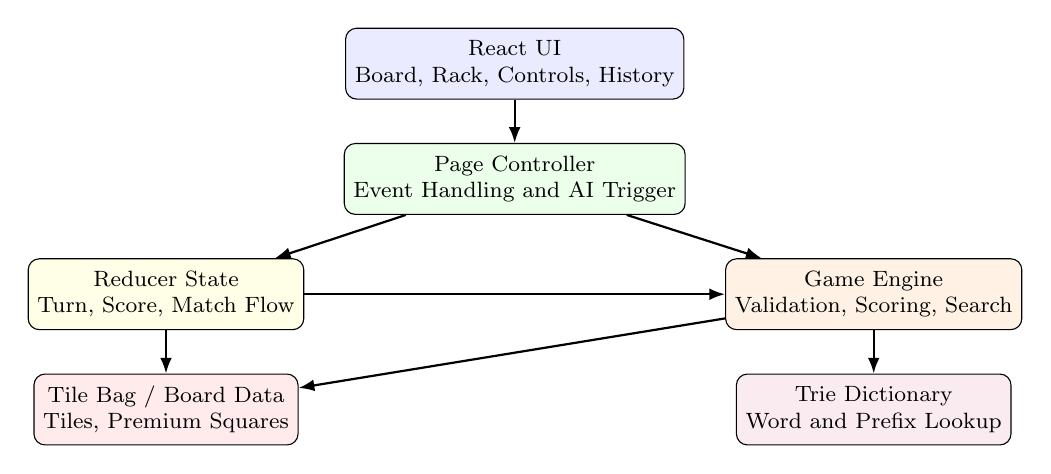
\begin{tikzpicture}[
node distance=0.55cm and 0.5cm,
box/.style={draw, rounded corners, align=center, minimum width=2.5cm, minimum height=0.9cm, font=\footnotesize},
arrow/.style={-{Latex[length=2mm]}, thick}
]
\node[box, fill=blue!8] (ui) {React UI\\Board, Rack, Controls, History};
\node[box, fill=green!8, below=of ui] (page) {Page Controller\\Event Handling and AI Trigger};
\node[box, fill=yellow!10, below left=of page] (state) {Reducer State\\Turn, Score, Match Flow};
\node[box, fill=orange!10, below right=of page] (engine) {Game Engine\\Validation, Scoring, Search};
\node[box, fill=purple!8, below=of engine] (dict) {Trie Dictionary\\Word and Prefix Lookup};
\node[box, fill=red!8, below=of state] (bag) {Tile Bag / Board Data\\Tiles, Premium Squares};

\draw[arrow] (ui) -- (page);
\draw[arrow] (page) -- (state);
\draw[arrow] (page) -- (engine);
\draw[arrow] (engine) -- (dict);
\draw[arrow] (engine) -- (bag);
\draw[arrow] (state) -- (bag);
\draw[arrow] (state.east) -- ++(0.7,0) |- (engine.west);
\end{tikzpicture}
\caption{High-level system architecture of Smart Scrabble.}
\label{fig:architecture}
\end{figure}

The presentation layer is responsible for rendering the board, rack, controls, score display, game-over screen, and move history. The top-level page component coordinates user actions and triggers AI turns. Because the game is highly interactive, the page runs as a client component.

The game engine layer contains the core logic of the application. It is divided into the following modules:
\begin{itemize}
\item \texttt{types.ts}: shared data structures such as tiles, placements, moves, and game state.
\item \texttt{constants.ts}: board size, rack size, tile distributions, point values, and premium square layout.
\item \texttt{board.ts}: board construction, placement validation, anchor detection, cross-check generation, and word extraction.
\item \texttt{tileBag.ts}: creation and shuffling of the tile bag, drawing tiles, and refilling racks.
\item \texttt{scoring.ts}: score calculation for the main word, cross words, letter multipliers, word multipliers, and bingo bonus.
\item \texttt{trie.ts}: dictionary loading and trie-based word lookup.
\item \texttt{moveGenerator.ts}: generation of legal candidate moves using anchor-based search and depth-first exploration.
\item \texttt{aiGreedy.ts}: immediate score maximization.
\item \texttt{aiHeuristic.ts}: weighted evaluation beyond raw score.
\item \texttt{gameState.ts}: reducer-driven turn and match management.
\end{itemize}

This separation is one of the main strengths of the project. The user interface does not directly implement game rules. Instead, it dispatches actions and calls engine functions, which keeps rule handling centralized and reduces duplication.

\section{Data Representation}
Several design decisions were made to keep the internal state explicit and easy to manipulate. Each board cell stores its row and column, the tile currently occupying the cell if any, the premium-square type, and whether the premium was already consumed. Each tile stores a letter, point value, and unique identifier. Using unique tile identifiers is useful because multiple tiles may have the same letter; tile identity matters when removing placements from a rack or applying a move.

The complete game state includes the board, two players, the current player index, the remaining tile bag, move history, the current temporary placements for the active turn, the selected AI strategy, status messages, and a flag indicating whether the AI is currently thinking. This structure makes the reducer pattern natural because every turn-related transition can be expressed as a state transformation.

\section{Dictionary Handling with a Trie}
Word validation is central to Scrabble. A naive implementation could store words in a hash set and test only complete words. However, move generation needs efficient prefix queries as well, since many partial strings are created while exploring possible placements. For that reason, the project uses a trie, also known as a prefix tree.

The dictionary is loaded from a JSON file in the public assets and inserted into a trie structure when the game starts. Once loaded, the trie is stored globally and reused throughout the session. The trie supports three main operations:
\begin{enumerate}
\item exact word lookup,
\item prefix existence queries, and
\item retrieval of valid continuation letters.
\end{enumerate}

The time complexity of searching a word or prefix is proportional to the length of that string rather than to the total dictionary size. This is especially useful during depth-first move generation, where the search repeatedly asks whether a partial sequence can still lead to a valid word. Without prefix pruning, the branching factor would become unnecessarily large.

\section{Move Generation Strategy}
Generating legal Scrabble moves is the most algorithmically demanding part of the project. The total number of possible placements is enormous if every empty square and every rack permutation are considered directly. To reduce this search space, the implementation follows an anchor-based strategy inspired by classical Scrabble literature \cite{appel1988fastest,gordon1994faster}.

An anchor is an empty square adjacent to at least one existing tile. In non-empty board states, any legal new move must interact with the board through such points. Therefore, instead of exploring all empty cells, the algorithm first collects anchors and then tries to construct words through them.

The move generator works in several stages:
\begin{enumerate}
\item If the board is empty, it generates first moves that pass through the center square.
\item Otherwise, it finds all anchor points.
\item For each anchor, it attempts horizontal and vertical expansion.
\item It builds optional prefixes before the anchor when space permits.
\item It extends the word forward with depth-first search.
\item At each step, it uses trie prefix checks to prune invalid partial strings.
\item For perpendicular interactions, it computes cross-check sets so that only letters that form valid cross words are allowed.
\item Valid finished moves are scored and stored.
\item Duplicate moves are removed before returning the result set.
\end{enumerate}

\begin{figure}[t]
\centering
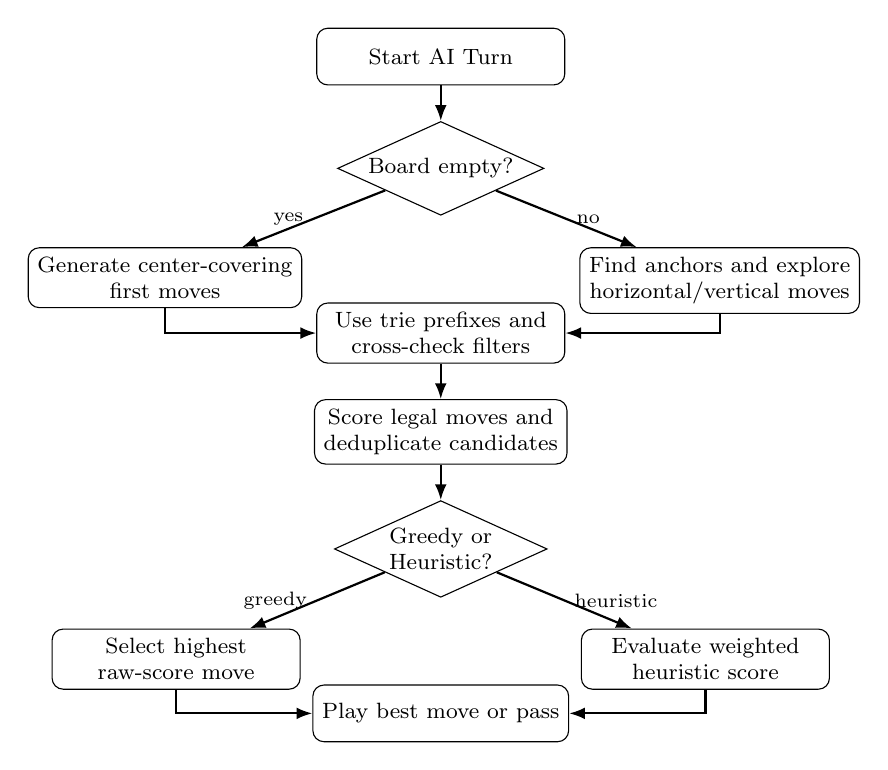
\begin{tikzpicture}[
node distance=0.45cm,
proc/.style={draw, rounded corners, align=center, minimum width=3.15cm, minimum height=0.72cm, font=\footnotesize},
decision/.style={draw, diamond, aspect=2.2, align=center, inner sep=1pt, font=\footnotesize},
arrow/.style={-{Latex[length=2mm]}, thick}
]
\node[proc] (start) {Start AI Turn};
\node[decision, below=of start] (empty) {Board empty?};
\node[proc, below left=0.7cm and 1.1cm of empty] (first) {Generate center-covering\\first moves};
\node[proc, below right=0.7cm and 1.1cm of empty] (anchors) {Find anchors and explore\\horizontal/vertical moves};
\node[proc, below=1.1cm of empty] (prefix) {Use trie prefixes and\\cross-check filters};
\node[proc, below=of prefix] (score) {Score legal moves and\\deduplicate candidates};
\node[decision, below=of score] (agent) {Greedy or\\Heuristic?};
\node[proc, below left=0.7cm and 1.1cm of agent] (greedy) {Select highest\\raw-score move};
\node[proc, below right=0.7cm and 1.1cm of agent] (heur) {Evaluate weighted\\heuristic score};
\node[proc, below=1.1cm of agent] (play) {Play best move or pass};

\draw[arrow] (start) -- (empty);
\draw[arrow] (empty) -- node[left, font=\scriptsize] {yes} (first);
\draw[arrow] (empty) -- node[right, font=\scriptsize] {no} (anchors);
\draw[arrow] (first) |- (prefix);
\draw[arrow] (anchors) |- (prefix);
\draw[arrow] (prefix) -- (score);
\draw[arrow] (score) -- (agent);
\draw[arrow] (agent) -- node[left, font=\scriptsize] {greedy} (greedy);
\draw[arrow] (agent) -- node[right, font=\scriptsize] {heuristic} (heur);
\draw[arrow] (greedy) |- (play);
\draw[arrow] (heur) |- (play);
\end{tikzpicture}
\caption{Flowchart of the AI move-generation and decision pipeline.}
\label{fig:flowchart}
\end{figure}

This approach is more efficient than unrestricted permutation search because it uses the board structure to narrow the search. In addition, the generator includes practical limits such as a maximum number of moves and a soft time limit. These limits help preserve responsiveness in the browser, especially when the AI is asked to consider many possibilities.

\section{Rule Enforcement and Scoring}
Legal move handling is implemented in a way that mirrors the flow of a real Scrabble turn. The player first places one or more tiles temporarily. Before submission, the system validates that:
\begin{itemize}
\item all positions are inside the board,
\item no occupied cell is overwritten,
\item all placed tiles lie in one row or one column,
\item there are no gaps between placed tiles after considering existing board tiles,
\item the first move covers the center square, and
\item later moves connect to the existing board.
\end{itemize}

If validation succeeds, the engine extracts the main word and all cross words formed by the move. All of them must exist in the dictionary for the move to be accepted. This design prevents illegal side effects such as accidentally forming an invalid perpendicular word.

Score calculation is handled separately from move validation. The scoring module applies letter multipliers and word multipliers only to newly placed tiles, while pre-existing tiles contribute their base values. It also handles cross words and awards the standard bingo bonus when all seven rack tiles are used in one turn. Separating scoring from validation makes the logic easier to reason about and keeps responsibilities clear.

\section{AI Design}
\subsection{Greedy Baseline}
The first AI agent is intentionally simple. It generates all legal moves and chooses the one with the highest immediate score. This greedy strategy provides a useful baseline. It is easy to explain, easy to implement, and often strong enough to produce credible play in casual settings.

However, greedy play has a known weakness: it does not consider the long-term consequences of a move. A high-scoring move may expose valuable premium squares, leave an unbalanced rack, or create many opportunities for the opponent. For this reason, the project also includes a second strategy.

\subsection{Heuristic Agent}
The heuristic AI evaluates each legal move using a weighted scoring function. Instead of looking only at the turn score, it combines multiple indicators of strategic quality:
\begin{itemize}
\item raw move score,
\item premium-square exposure penalty,
\item reward for using more tiles,
\item rack balance after the move,
\item proximity to the board center, and
\item penalty for opening too many new anchor points.
\end{itemize}

The heuristic function used in the implementation can be summarized as
\begin{align}
E(m) ={}& w_s S(m) + w_b B(m) + w_t T(m) \nonumber\\
&+ w_r R(m) + w_c C(m) + w_o O(m).
\end{align}
Here, $S(m)$ is the raw score, $B(m)$ reflects premium exposure, $T(m)$ measures tile usage, $R(m)$ captures rack balance, $C(m)$ measures center proximity, and $O(m)$ estimates board openness. Negative weights are assigned to factors that increase opponent opportunity, while positive weights reward locally desirable behavior.

This is not a learned model. The weights were chosen manually to encode reasonable Scrabble intuitions, following the general idea of evaluation-function design used in board-game AI and Scrabble engines such as Maven \cite{sheppard2002world}. Even so, the heuristic agent tends to produce more balanced moves than the greedy baseline because it accounts for positional side effects.

\subsection{Practical AI Turn Handling}
AI computation is triggered automatically when the current player is the computer. The application delays the visible ``thinking'' indicator slightly so that very fast turns do not flash distracting UI updates. Candidate generation for the greedy and heuristic agents uses modest search bounds to keep interaction smooth in the browser.

\section{User Interface and Interaction Design}
Although the main focus of the project is algorithmic, the user interface is also important because the game is meant to be played directly by a user. The interface includes the board, rack, control buttons, status messages, score board, move history, and a game-over dialog. The current version also places move history in a dedicated side panel for easier reading during longer games.

The visual language follows a traditional board-game style with dark backgrounds and wood-like tile presentation. The use of Tailwind CSS provides fast layout control, while CSS modules allow the board to keep its own isolated styling. The application is structured so that the main board interaction remains in the center, while information panels such as score and history are accessible without covering the board.

The game begins with a start screen where the user chooses the AI difficulty. During play, the user selects a tile from the rack and places it on the board. Temporary placements can be recalled before submission. Once a move is submitted, the game validates it and either accepts it or shows a message explaining why it is invalid. This immediate feedback improves usability and helps players understand the rules enforced by the system.

\section{Reducer-Based State Management}
The project uses a reducer to manage the full game state. This decision is appropriate because the game contains many state transitions that are interdependent: placing a tile affects the rack, submitting a move affects the board and score, passing changes the turn counter, exchanging tiles modifies both rack and bag, and end-game logic depends on multiple conditions.

The reducer pattern makes each transition explicit through action types such as \texttt{PLACE\_TILE}, \texttt{SUBMIT\_MOVE}, \texttt{PASS\_TURN}, and \texttt{AI\_MOVE}. This style has three practical benefits:
\begin{enumerate}
\item it centralizes game transitions,
\item it reduces accidental inconsistencies between UI state and engine state, and
\item it makes future testing easier because actions can be replayed systematically.
\end{enumerate}

For a project of this size, a reducer is simpler and more appropriate than introducing a larger external state library.

\section{Observed Results}
The system succeeds in its primary objective: it provides a complete and playable Scrabble experience against two different AI opponents inside the browser. In informal use, the greedy AI behaves predictably and often chooses flashy high-scoring moves, which makes it easy to understand as a baseline. The heuristic AI generally produces more controlled play by avoiding some moves that are attractive in the short term but risky in board structure.

From a software perspective, the move generator and trie combination make the game responsive enough for interactive use. The interface remains understandable because the game state and the visual presentation are clearly separated. The move history also helps players inspect the sequence of play and compare the behavior of the two AI strategies.

The project therefore demonstrates that even within a course-scale implementation, it is possible to combine a web application framework with nontrivial game AI techniques in a clean and usable way.

\begin{table}[t]
\caption{Configured AI search budgets in the current implementation}
\label{tab:budgets}
\centering
\begin{tabular}{lcc}
\toprule
Agent & Time limit & Candidate cap \\
\midrule
Greedy & 250 ms & 2500 moves \\
Heuristic & 400 ms & 3500 moves \\
\bottomrule
\end{tabular}
\end{table}

\begin{table}[t]
\caption{Compact evaluation template for human-vs-AI match logging}
\label{tab:matchlog}
\centering
\begin{tabular}{>{\raggedright\arraybackslash}p{0.95cm} >{\raggedright\arraybackslash}p{1.2cm} >{\centering\arraybackslash}p{0.95cm} >{\centering\arraybackslash}p{1.4cm} >{\centering\arraybackslash}p{0.85cm}}
\toprule
Match & Opponent & Winner & Final score & Turns \\
\midrule
M1 & Greedy & Human/AI & H--A & \# \\
M2 & Heuristic & Human/AI & H--A & \# \\
M3 & Heuristic & Human/AI & H--A & \# \\
\bottomrule
\end{tabular}
\end{table}

\subsection{Evaluation Notes}
Table~\ref{tab:budgets} reports the actual search-budget parameters currently hard-coded in the system. These values explain why the AI remains interactive even in a browser setting and should be interpreted as engineering constraints rather than measured average runtimes. At the time of writing, the project does not yet include automated timing logs or a persistent match recorder; therefore, it would be misleading to report fabricated millisecond averages or invented win-loss records.

For that reason, Table~\ref{tab:matchlog} is included as a compact evaluation template for manual or scripted experiments. A stronger final version of the report should populate this table with several complete human-vs-AI matches and add summary statistics such as average move-generation time, average score, and win rate by agent type.

\section{Limitations}
The current system still has several limitations. First, the AI is heuristic rather than adversarial. It does not use minimax, Monte Carlo methods, or opponent modeling, so it cannot reason deeply about future counterplay. Second, the heuristic weights were selected manually and were not tuned through data-driven evaluation. Third, the move generator is bounded by practical time and move limits, which is good for responsiveness but may miss some stronger candidates in difficult positions.

Another limitation is that the project prioritizes interactive completeness over competitive strength. The implementation is suitable for a course project and casual gameplay, but it is not intended to compete with advanced Scrabble engines such as Maven \cite{sheppard2002world}. Additionally, the current codebase would benefit from more systematic automated tests and a clearer quantitative evaluation protocol.

There is also room for future cleanup in locale and dictionary handling. Some parts of the codebase contain Turkish-specific letter normalization and distributions, while the user-facing description refers to English dictionary play. A future revision should make the language setting explicit and keep the dictionary, tile distribution, and character normalization fully consistent.

\section{Future Work}
Several extensions would significantly improve the project:
\begin{itemize}
\item add automated unit and integration tests for rule validation, scoring, and AI behavior;
\item implement stronger AI using minimax with alpha-beta pruning or simulation-based search;
\item support multiple dictionary packs and explicit language selection;
\item add rack exchange selection instead of exchanging the entire rack at once;
\item include performance instrumentation to measure move-generation time and branching behavior; and
\item deploy persistent match history or multiplayer functionality.
\end{itemize}

Among these, the most academically interesting next step would be a stronger look-ahead agent, while the most practical improvement would likely be better testing and language consistency.

\section{Conclusion}
Smart Scrabble demonstrates how a traditional board game can be implemented as a modern browser application while still containing meaningful algorithmic content. The project combines a clean TypeScript and Next.js frontend with a modular game engine, trie-based dictionary validation, anchor-based move generation, formal score computation, and two AI strategies of different sophistication.

The greedy and heuristic agents offer a useful comparison between immediate-score optimization and multi-factor strategic evaluation. Although the system is not intended as a professional-level Scrabble engine, it successfully captures many of the core technical ideas behind word-game AI in an accessible and playable form. As a term project, it provides both a functional software artifact and a strong foundation for future experimentation in search, heuristics, and game intelligence.

\bibliographystyle{IEEEtran}
\bibliography{smart_scrabble_refs}

\end{document}
